\documentclass[10pt,a4paper]{article}
\usepackage[margin=18mm]{geometry}
\usepackage[T1]{fontenc}
\usepackage[utf8]{inputenc}
\usepackage{lmodern}
\usepackage{microtype}
\usepackage{graphicx}
\usepackage{booktabs}
\usepackage{array}
\usepackage{tabularx}
\usepackage{longtable}
\usepackage{multicol}
\usepackage{amsmath}
\usepackage{placeins}
\newcolumntype{L}[1]{>{\raggedright\arraybackslash}p{#1}}
\newcolumntype{Y}{>{\raggedright\arraybackslash}X}
\setlength{\tabcolsep}{5pt}
\renewcommand{\arraystretch}{1.08}
\setlength{\textfloatsep}{8pt}
\renewcommand{\topfraction}{0.95}
\renewcommand{\textfraction}{0.05}
\renewcommand{\floatpagefraction}{0.85}
\setlength{\intextsep}{9pt}
\setlength{\emergencystretch}{2em}
\usepackage{float}
\usepackage{xcolor}
\usepackage{hyperref}
\usepackage[numbers,sort&compress]{natbib}
\usepackage{caption}
\usepackage{subcaption}
\usepackage{enumitem}
\setlist{nosep,topsep=4pt}
\hypersetup{colorlinks=true,linkcolor=blue!55!black,citecolor=blue!55!black,urlcolor=blue!55!black}
\setlength{\parskip}{0.2em}
\setlength{\parindent}{0pt}
\captionsetup{font=small,labelfont=bf,skip=4pt}
\newcommand{\metric}[1]{\texttt{#1}}
\title{Counterfactual Background Reconstruction for Realistic Camouflaged Object Detection\\[0.4em]
\large Project Progress, Full-Split Evaluation, and Critical Assessment}
\author{Master's Research Project Report}
\date{Prepared for thesis-advisor review\\3 October 2026}

\begin{document}
\hypersetup{pageanchor=false}\begin{titlepage}
\centering
{\Large\bfseries Counterfactual Background Reconstruction\\for Realistic Camouflaged Object Detection\par}
\vspace{0.5em}
{\large Executive summary for thesis-advisor review\par}
{\small 3 October 2026\par}
\vspace{1.4em}
\raggedright
\textbf{Research question.} Can reconstructing a plausible background after removing a frozen COD model's candidate provide useful evidence for distinguishing camouflage, empty background, and salient non-camouflaged objects? The project tests this through SINet-V2 candidates, LaMa reconstruction, and appearance, learned-feature, and structural residuals, followed by verification and optional refinement.

\medskip
\textbf{Headline findings on the saved official evaluation split.}
\begin{itemize}[leftmargin=1.4em,itemsep=0.65em]
\item \textbf{Three-way accuracy: 0.7122}; macro-F1: \textbf{0.7018}, on 3,600 USC12K images. The saved split is named \texttt{usc12k\_official\_val}.
\item \textbf{Negative false acceptance: 1.0000 $\rightarrow$ 0.2883}. The baseline comparison defines any nonempty raw candidate as accepted; verification rejects many negative scenes but also rejects some true CO images.
\item \textbf{Segmentation tradeoff:} raw SINet-V2 masks remain best on PySODMetrics S-alpha, weighted F-beta, and adaptive E-measure. Verification has only a small MAE advantage; refinement does not provide an overall CO segmentation improvement.
\end{itemize}
\medskip
\textbf{What the calibration revealed.} The initial appearance/structural rule failed the source-matched diagnostic; a COD10K-calibrated feature cutoff inverted on USC12K salient-object negatives. A feature-only band, calibrated on USC12K training-derived samples, was frozen before the full evaluation, but source/class confounding remains unresolved.

\medskip
\textbf{Thesis claim.} The verifier succeeds as a candidate rejection mechanism on this evaluated split, while the evidence does not show that it improves CO segmentation or generalizes independently of dataset source.

\medskip
\textbf{Assessment.} This supports a substantive master's thesis as an audited empirical study of counterfactual verification, dataset shortcuts, and the rejection--segmentation tradeoff. A claim of state-of-the-art performance, source-independent camouflage recognition, or improved segmentation is not supported.

\vfill
{\small All headline results are supported by Tables~\ref{tab:classification}--\ref{tab:pysod} and the exact saved artifacts mapped in Appendix~\ref{app:provenance}. The six supplementary examples are illustrations selected by outcome, not a new performance estimate.}
\end{titlepage}\hypersetup{pageanchor=true}\pagenumbering{arabic}

\begin{abstract}
This report documents the complete proposal-to-evaluation path for a post-hoc counterfactual verification layer for realistic camouflaged-object detection (COD). The system starts from a frozen SINet-V2 candidate mask, removes and inpaints the candidate region with LaMa, and scores the difference between the original image and its reconstructed-background counterfactual. Early experiments exposed serious source/class confounding: appearance and structural fusion did not transfer even to a small COD10K-matched negative set, and a feature-only direction selected on COD10K inverted on USC12K salient-object negatives. A frozen two-cut band was therefore calibrated on small USC12K training-derived samples and then applied to the saved official evaluation manifest. The full split yielded three-way accuracy \(0.7122\), macro-F1 \(0.7018\), and negative false acceptance \(0.2883\), with class-stratified bootstrap intervals reported below. A final independent metric check with PySODMetrics shows that the verifier and the refinement output do not improve CO segmentation quality over the raw SINet-V2 masks: raw masks have the best S-alpha, weighted F-beta, and adaptive E-measure, while verification has only a very small MAE advantage. The project therefore provides a useful, carefully audited investigation of open-world failure modes and a measurable negative-rejection add-on, but it does not establish a new state-of-the-art segmenter or source-independent camouflage detector.

All project-result numbers are traceable through Appendix~\ref{app:provenance}; full precision is retained in the accompanying CSV/JSON files. A supplementary evaluation exported previews for six previously selected examples, reusing all six saved reconstruction/residual caches without new model inference.
\end{abstract}

\begingroup\small\setcounter{tocdepth}{1}
\begin{multicols}{2}\tableofcontents\end{multicols}\endgroup

\section{Introduction and recap}
\subsection{Research question and proposed pipeline}
The proposal asks whether a candidate object can be tested counterfactually: if the candidate is removed and the surrounding scene is plausibly reconstructed, does the discrepancy between the original image and the reconstructed image provide evidence that the candidate is camouflaged? The proposed pipeline is
\[
 I \longrightarrow M_0 \longrightarrow \hat I_{bg} \longrightarrow R \longrightarrow M_{final},
\]
where \(I\) is the input, \(M_0\) is the initial frozen detector mask, \(\hat I_{bg}\) is an inpainted image after the candidate region has been masked, \(R\) is a residual evidence representation, and \(M_{final}\) is the retained or refined mask. The proposal's hypothesis is that a real camouflaged object may blend into the scene enough that its removal produces a different residual signature from a salient non-camouflaged object or a scene with no foreground object. The intended contribution was an empirical analysis of residual types and an evaluation of their use in negative rejection and mask refinement, not a new inpainting architecture. The original proposal is the project source for these questions. [Source: supplied proposal file, \texttt{project\_proposal\_draft\_4.pdf}]

\subsection{Why USC12K replaced OPC16K}
OPC16K was the proposal's preferred realistic benchmark. At the time this project recorded its acquisition status, the OPC16K authors' repository listed its public release as forthcoming; the archive was therefore not available through the project's official-source-only download procedure. USC12K had an author-provided image/annotation release and supported a full saved evaluation, so it became the practical benchmark. The report does not claim that OPC16K remains unavailable today; the status statement is limited to the project's acquisition record. RCOD was also downloaded, but its annotations are object-detection boxes rather than the pixel masks required for this project's segmentation/refinement experiments. \citep{opc16k,usc12k,rcod}


\section{Methodology}
\subsection{Dataset and evaluation protocol}
The saved manifest contains 3,600 USC12K examples: 1,800 CO, 900 BG, and 900 NOCOD. The manifest's split field is \texttt{usc12k\_official\_val}, and the dataset builder derives this evaluation split from the official \texttt{val.txt} list. To avoid ambiguity, this report calls it the \emph{official evaluation split}; it does not rename it an official test split. The image labels map the dataset's four scenes as follows: Scene A to NOCOD, Scene B to CO, Scene C to CO because camouflage is present alongside salient content, and Scene D to BG. The published USC12K dataset explicitly includes scenarios for salient and camouflaged objects in unconstrained scenes; the project's label mapping is a project-specific reduction to the three requested classes. \citep{usc12k}


The split was evaluated and inspected before this report. Consequently, the confidence intervals below quantify image resampling variability within this already-inspected split. They do not turn it into a fresh blind test, correct for source shift, or justify choosing a model after looking at the results. The saved post-hoc analysis itself marks this limitation explicitly.


\subsection{Frozen baseline, reconstruction, and residuals}
The raw candidate generator is the frozen SINet-V2 COD segmentation model; this project did not retrain it. For each image, the candidate mask is dilated by 5 pixels and passed to the LaMa inpainting backend, which fills the masked area and yields \(\hat I_{bg}\). LaMa is used as a counterfactual reconstruction tool, not as evidence that the reconstructed image is a unique or ground-truth background. The saved full run used the LaMa ONNX backend on CPU. The frozen feature residual uses an ImageNet-pretrained ResNet-18 layer2 representation: the original image and \(\hat I_{bg}\) are resized to 256 by 256, normalized, embedded, and compared by cosine distance. \citep{sinetv2,lama}


The system implemented three residual signals. Appearance is mean absolute RGB difference in the candidate region; feature is the cosine distance between frozen ResNet-18 layer2 embeddings; structural is a discrepancy between Canny edge maps. The combined residual was initially an equal-weight or calibrated scalar score, but it is not a probability. The final decision uses only the feature residual, with appearance and structural weights set to zero. The three-way rule is: predict BG for score below 0.185, predict CO for score from 0.185 through 0.285 inclusive, and predict NOCOD above 0.285. A predicted CO retains the candidate; a BG or NOCOD decision suppresses it. These cut points are train-derived choices, not universal thresholds. The CO measures used in this report follow standard foreground-map evaluation protocols and are recomputed with PySODMetrics. \citep{sm,wfm,em,pysod}


\begin{figure}[htbp]
\centering
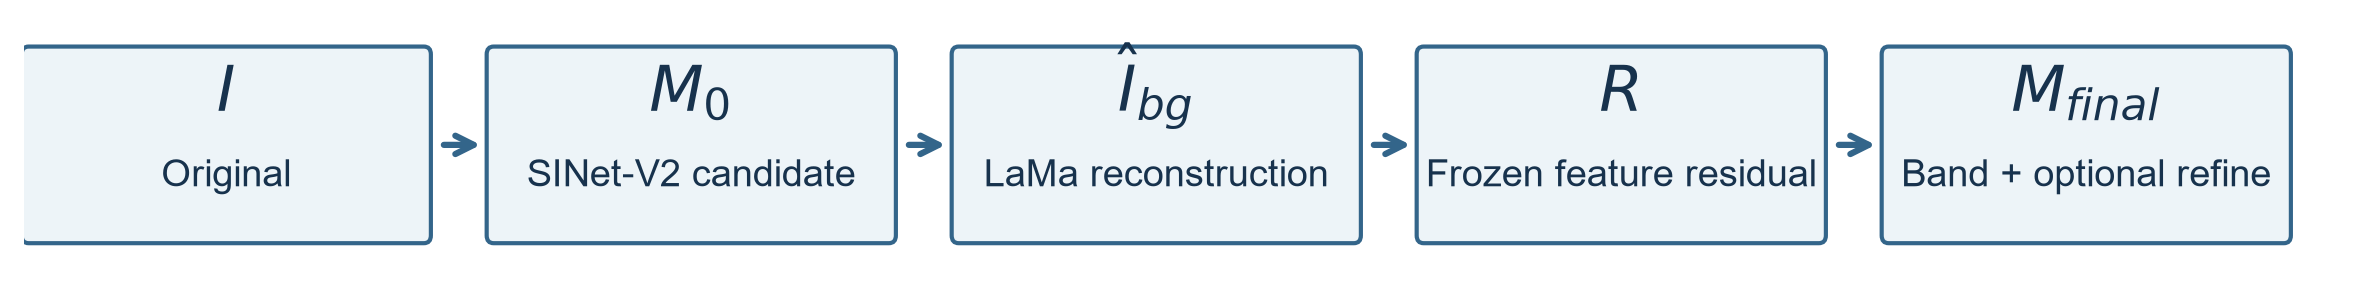
\includegraphics[width=\textwidth]{figures/pipeline.png}
\caption{Counterfactual reconstruction and feature-band verification pipeline.}
\label{fig:pipeline}

\end{figure}

\subsection{Calibration journey and pitfalls}
Table~\ref{tab:calibration} preserves the complete progression from the initial composite through source-matched diagnostics, the feature-only transfer failure, and the final USC12K band. The apparent composite success did not survive source matching, and the CO--NOCOD inversion rules out treating one binary score direction as universal. The final train-derived band and disjoint holdout support further investigation, but their small size and persistent source/class association do not establish source-independent generalization (Appendix~\ref{app:provenance}).

\begin{table}[htbp]
\centering
\caption{Calibration, source-matched diagnostics, and frozen-rule checks.}
\label{tab:calibration}
\small
\begin{tabularx}{\textwidth}{L{3.35cm}rL{2.0cm}rrY}
\toprule
\textbf{Stage / sample} & \textbf{$n$} & \textbf{Measure $\uparrow$} & \textbf{Value} & \textbf{95\% CI} & \textbf{Interpretation} \\
\midrule
Initial composite (20/class) & 60 & Tuning accuracy & 0.817 & -- & Source pools fully confounded. \\
COD10K matched (25/class) & 50 & Low-score AUC & 0.424 & [0.270, 0.587] & Frozen composite failed. \\
Feature on matched diagnostic & 50 & High-score AUC & 0.902 & -- & Promising only on this source pair. \\
Fresh feature development (25/class) & 50 & Tuning accuracy & 0.800 & -- & COD10K proxy; transfer unproven. \\
USC CO vs NOCOD (15/class) & 30 & High-score AUC & 0.093 & [0.000, 0.227] & Strong direction inversion. \\
USC band calibration (40/class) & 120 & Accuracy / F1 & 0.708 / 0.709 & -- & Training tuning result. \\
USC frozen holdout (15/class) & 45 & Accuracy / F1 & 0.667 / 0.672 & -- & Disjoint but still source-confounded. \\
\bottomrule
\end{tabularx}
\par\smallskip{\footnotesize Initial rule: low-score CO at 0.10; appearance/feature/structural weights 0.25/0/0.75. Fresh feature rule: high-score CO at 0.175. Final band: 0.185/0.285. F1 denotes macro-F1. These are distinct small samples; tuning scores are not unbiased test estimates.}
\end{table}


\subsection{Runtime and compute caveat}
The full verifier processed the saved 3,600-row manifest with no residual-cache hits. Its saved mean time was 6.067924718557107 seconds per image, including mean inpainting time of 5.597485009890128 seconds per image; total time was 22,164.16736839991 seconds. This is not a lightweight runtime in an absolute sense on the available CPU. The refinement pass was much shorter because it reused 3,600 cached residuals; that cached timing must not be confused with a clean end-to-end runtime. The phrase ``lightweight add-on'' refers to the small frozen post-hoc decision rule and no extra learned segmenter training, not low wall-clock cost when fresh inpainting is required.


\section{Results}
\subsection{Three-way classification on the saved official evaluation split}
The final rule produced three-way accuracy 0.7122222 and macro-F1 0.7018039. The class-specific recalls were 0.6833333 for BG, 0.7594444 for CO, and 0.6466667 for NOCOD. The reported class-stratified image-bootstrap intervals use 2,000 replicates and seed 20261001. The intervals and saved full-split confusion matrix appear in Table~\ref{tab:classification} and Appendix~\ref{app:counts}; Figure~\ref{fig:confusion} visualizes the same saved counts. The dominant errors are CO-to-NOCOD (292 images) and BG-to-CO (270), so the classifier is not reliably resolving camouflage from salient-object negatives. Verify and refine share the same classifier outputs because refinement changes masks, not the feature-band class decision.

\begin{table}[htbp]
\centering
\caption{Feature-band classification on the official evaluation split.}
\label{tab:classification}
\small
\begin{tabular}{lrr}
\toprule
\textbf{Measure} & \textbf{Estimate $\uparrow$*} & \textbf{95\% CI} \\
\midrule
Three-way accuracy & 0.7122 & [0.6978, 0.7269] \\
Macro-F1 & 0.7018 & [0.6865, 0.7171] \\
Balanced accuracy & 0.6965 & [0.6809, 0.7122] \\
BG recall & 0.6833 & [0.6522, 0.7133] \\
CO recall & 0.7594 & [0.7389, 0.7811] \\
NOCOD recall & 0.6467 & [0.6156, 0.6778] \\
Negative false-acceptance rate & 0.2883 & [0.2678, 0.3089] \\
Negative rejection accuracy & 0.7117 & Not reported \\
Binary CO-vs-negative accuracy & 0.7356 & Not reported \\
CO acceptance rate & 0.7594 & [0.7389, 0.7811] \\
\bottomrule
\end{tabular}

\par\smallskip{\footnotesize Class-stratified 95\% intervals; unavailable intervals are marked ``Not reported. *False acceptance is the exception: lower is better ($\downarrow$). Full precision: Appendix~\ref{app:provenance}.}
\end{table}



\begin{figure}[htbp]
\centering
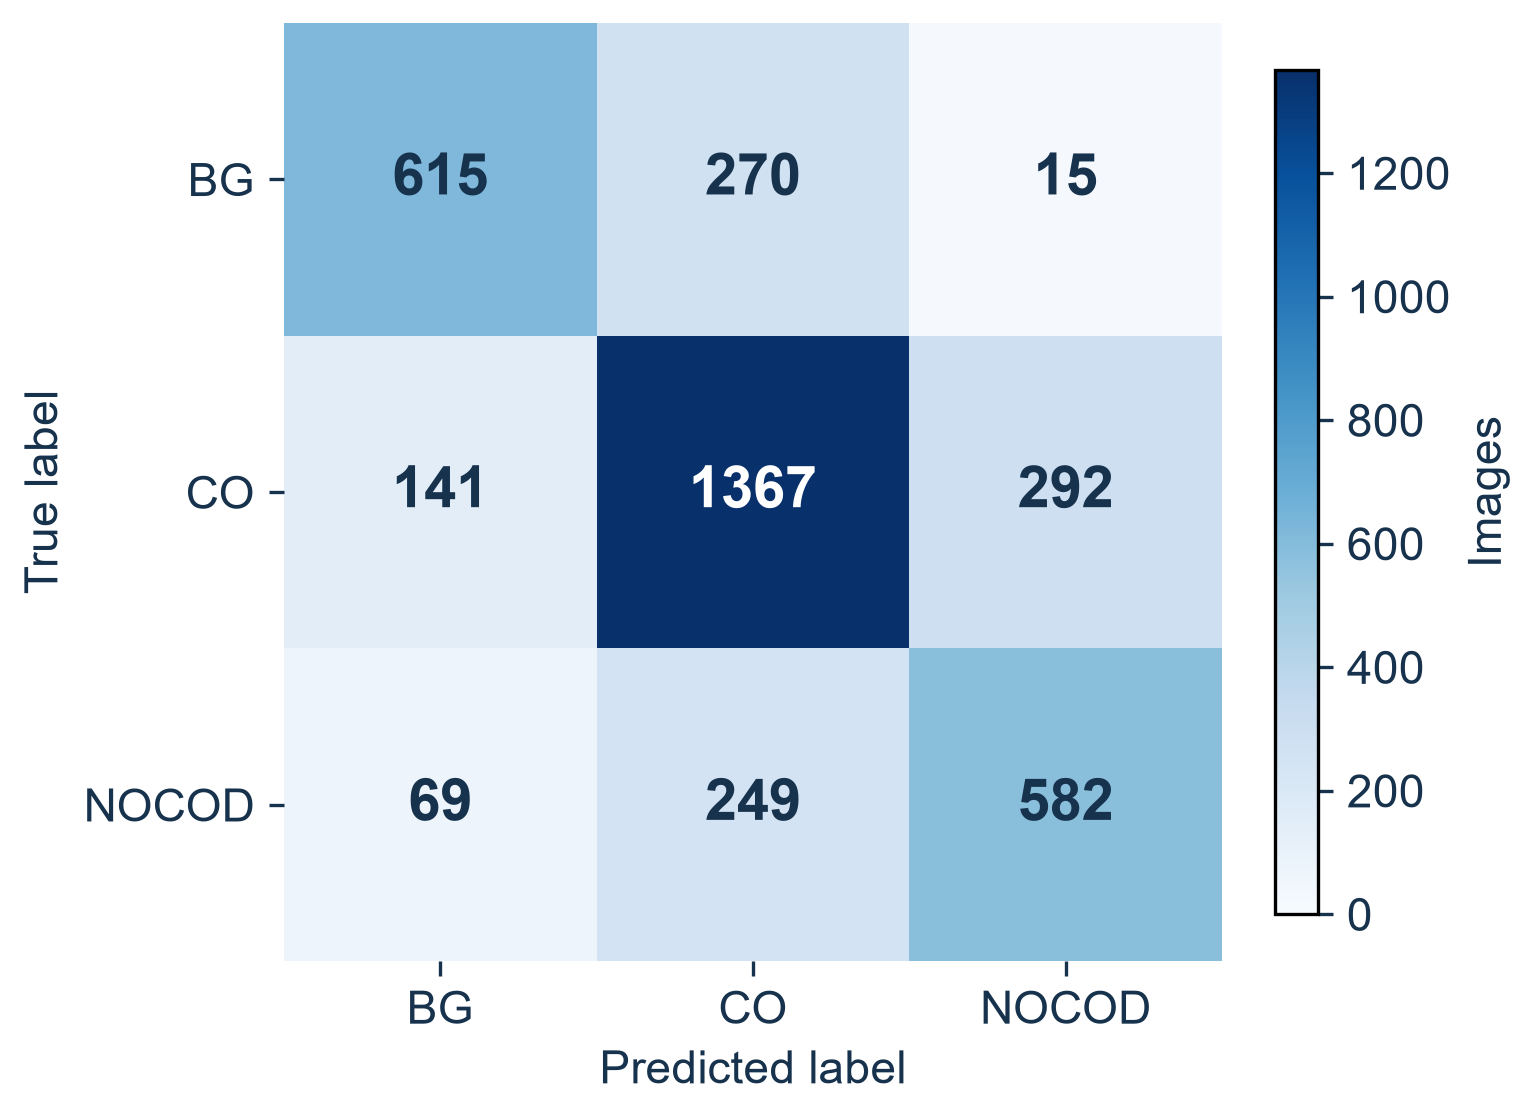
\includegraphics[width=0.53\textwidth]{figures/confusion_matrix.png}
\caption{Full-split confusion matrix with true rows and predicted columns.}
\label{fig:confusion}

\end{figure}

\subsection{Negative rejection compared with raw candidate masks}
Without verification, every BG and NOCOD item in the saved manifest has a nonempty raw SINet-V2 candidate mask: the saved post-hoc per-image table contains 900 of 900 nonempty BG masks and 900 of 900 nonempty NOCOD masks. Under the explicit operational definition ``candidate mask is nonempty means accepted as an object,'' the raw baseline therefore falsely accepts 1,800 of 1,800 negative images (rate 1.0000). The feature-band verifier falsely accepts 0.2883333 of negative images (95\% stratified bootstrap CI 0.2677778--0.3088889), or rejects 0.7116667. The reduction is a real, useful negative-rejection result for this split. It comes with a CO acceptance rate of 0.7594444, so 0.2405556 of CO images are rejected. The binary CO-vs-negative accuracy is 0.7355556. This comparison concerns image-level acceptance; it does not claim better segmentation masks.

\begin{table}[htbp]
\centering
\caption{Negative acceptance and predicted-mask area by condition.}
\label{tab:negativearea}
\small
\begin{tabular}{llrr}
\toprule
\textbf{Condition} & \textbf{Class} & \textbf{False acceptance $\downarrow$} & \textbf{Area fraction $\downarrow$} \\
\midrule
Raw candidates & BG & 1.000 & 0.02855 \\
Raw candidates & NOCOD & 1.000 & 0.1255 \\
Feature-band verify & BG & 0.3 & 0.01755 \\
Feature-band verify & NOCOD & 0.2767 & 0.03281 \\
Feature-band refine & BG & 0.3 & 0.008545 \\
Feature-band refine & NOCOD & 0.2767 & 0.01705 \\
\bottomrule
\end{tabular}

\par\smallskip{\footnotesize Raw acceptance means any nonempty candidate. Area is the mean per-image mask fraction; classification decisions are identical for verify and refine.}
\end{table}


\subsection{CO segmentation: consistent PySODMetrics comparison}
The final table uses PySODMetrics 1.6.2 on the same saved CO masks and ground truths for raw, verify, and refine. Raw means saved SINet-V2 candidate masks with verification disabled. Verify suppresses candidate masks when the feature rule predicts BG or NOCOD. Refine additionally transforms the retained masks using cached residual maps; no SINet-V2 or LaMa inference was needed for this metric check. The internal project implementation previously gave misleading S-alpha and weighted F-beta values; canonical thesis reporting should use this consistent PySODMetrics table. Its adaptive E-measure is not the same implementation/protocol as the internal continuous \metric{E\_phi}. 

Raw masks have the best S-alpha, weighted F-beta, and adaptive E-measure. Verify reduces negative mask area and improves MAE by only 0.000160225 (raw 0.067364560 versus verify 0.067204336), while lowering the other three CO metrics. Refinement further lowers the reported S-alpha and weighted F-beta and raises MAE to 0.069261117; adaptive E-measure is 0.639741162, still below raw 0.720589303. Thus the detection/rejection layer reduces false-positive masks on negative images but harms aggregate target-present segmentation quality; the refinement branch does not deliver a general segmentation improvement under the consistently recomputed metrics.

\begin{table}[htbp]
\centering
\caption{CO segmentation evaluated consistently with PySODMetrics.}
\label{tab:pysod}
\small
\begin{tabular}{lrrrr}
\toprule
\textbf{Condition} & $\boldsymbol{S_\alpha\uparrow}$ & $\boldsymbol{F_\beta^w\uparrow}$ & $\boldsymbol{E_{adp}\uparrow}$ & \textbf{MAE $\downarrow$} \\
\midrule
Raw SINet-V2 baseline & 0.6959 & 0.4663 & 0.7206 & 0.06736 \\
Feature-band verify & 0.6537 & 0.3743 & 0.6198 & 0.0672 \\
Feature-band refine & 0.6037 & 0.2958 & 0.6397 & 0.06926 \\
\bottomrule
\end{tabular}

\par\smallskip{\footnotesize PySODMetrics 1.6.2; identical CO ground truths for all conditions. $E_{adp}$ is sample-based adaptive E-measure.}
\end{table}

Figure~\ref{fig:pysod} uses a separate vertical scale for each metric; higher is better for S-alpha, weighted F-beta and adaptive E, while lower MAE is better.

\begin{figure}[htbp]
\centering
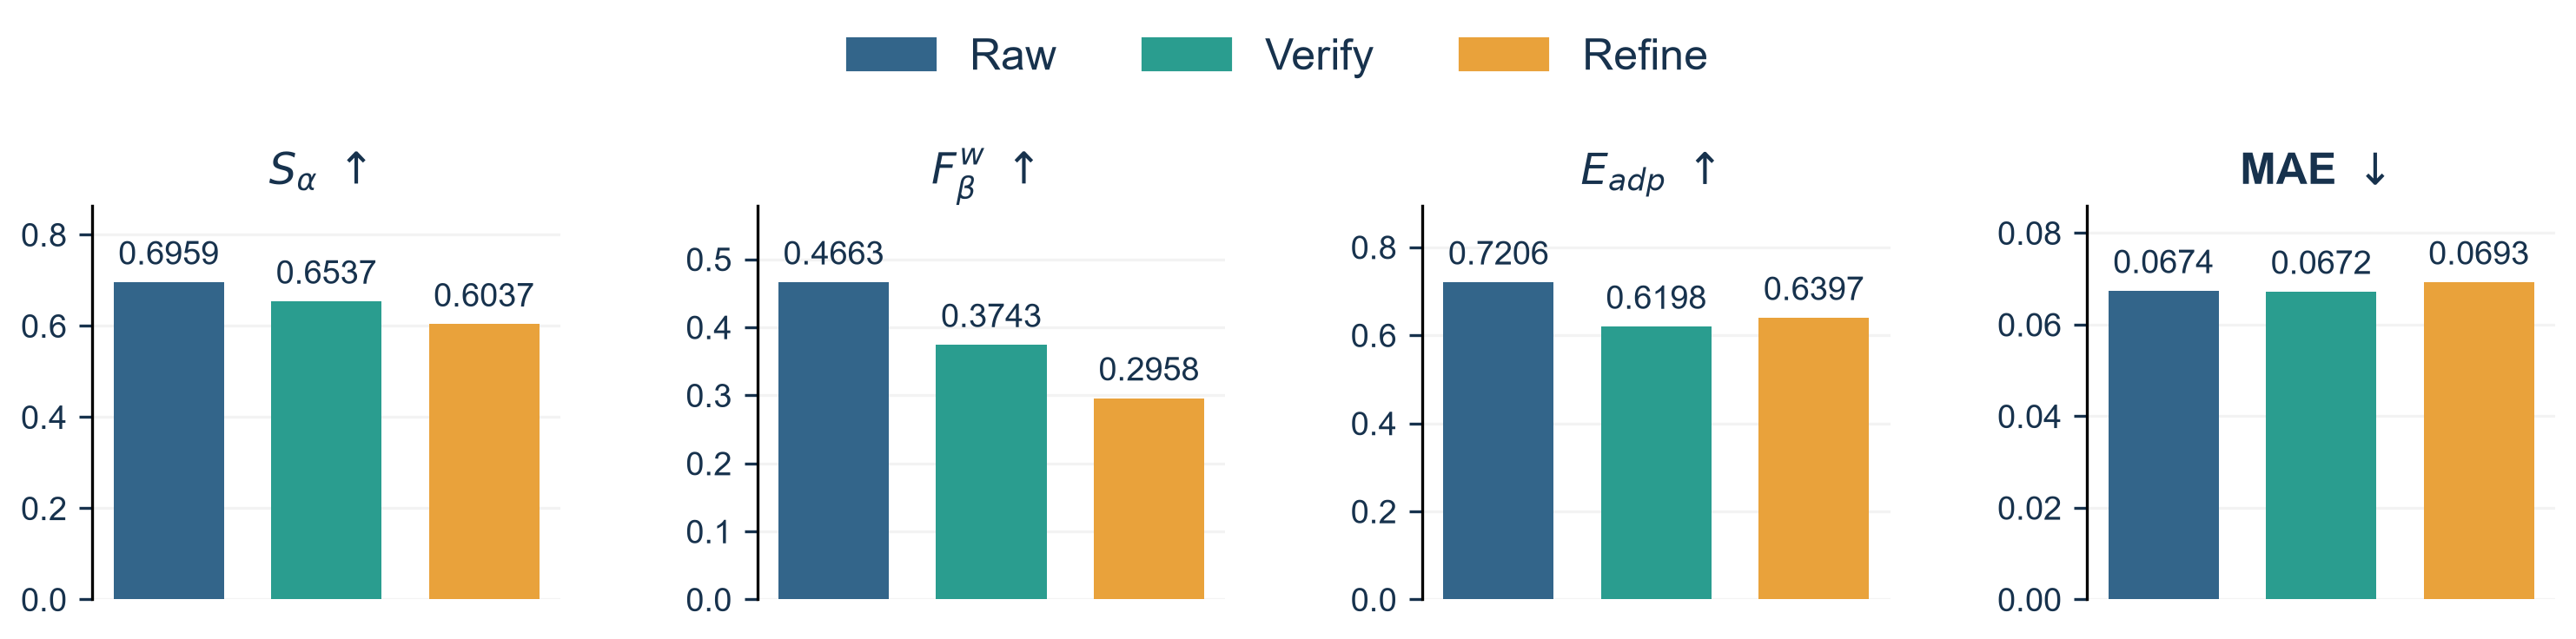
\includegraphics[width=\textwidth]{figures/pysodmetrics_grouped_bars.png}
\caption{PySODMetrics comparison for raw, verified, and refined CO masks.}
\label{fig:pysod}

\end{figure}

\subsection{Qualitative examples}
Figure~\ref{fig:qualitative} retains the same six previously selected examples: one correct and one incorrect class decision per class. A supplementary evaluation with \texttt{--save-previews} reused all six full-run caches; its recorded evaluation-loop time was 2.589 seconds, excluding startup. The displayed stages are original, candidate overlay, LaMa reconstruction, feature-residual heatmap (fixed scale), and the refined final mask; orange contours show CO ground truth. Row labels give true $\rightarrow$ predicted class. Images are letterboxed consistently without cropping or geometric distortion. These outcome-selected illustrations are not representative performance estimates; their decisions, scores, and mask areas were checked against the saved full run (Appendix~\ref{app:provenance}).

\begin{figure}[htbp]
\centering
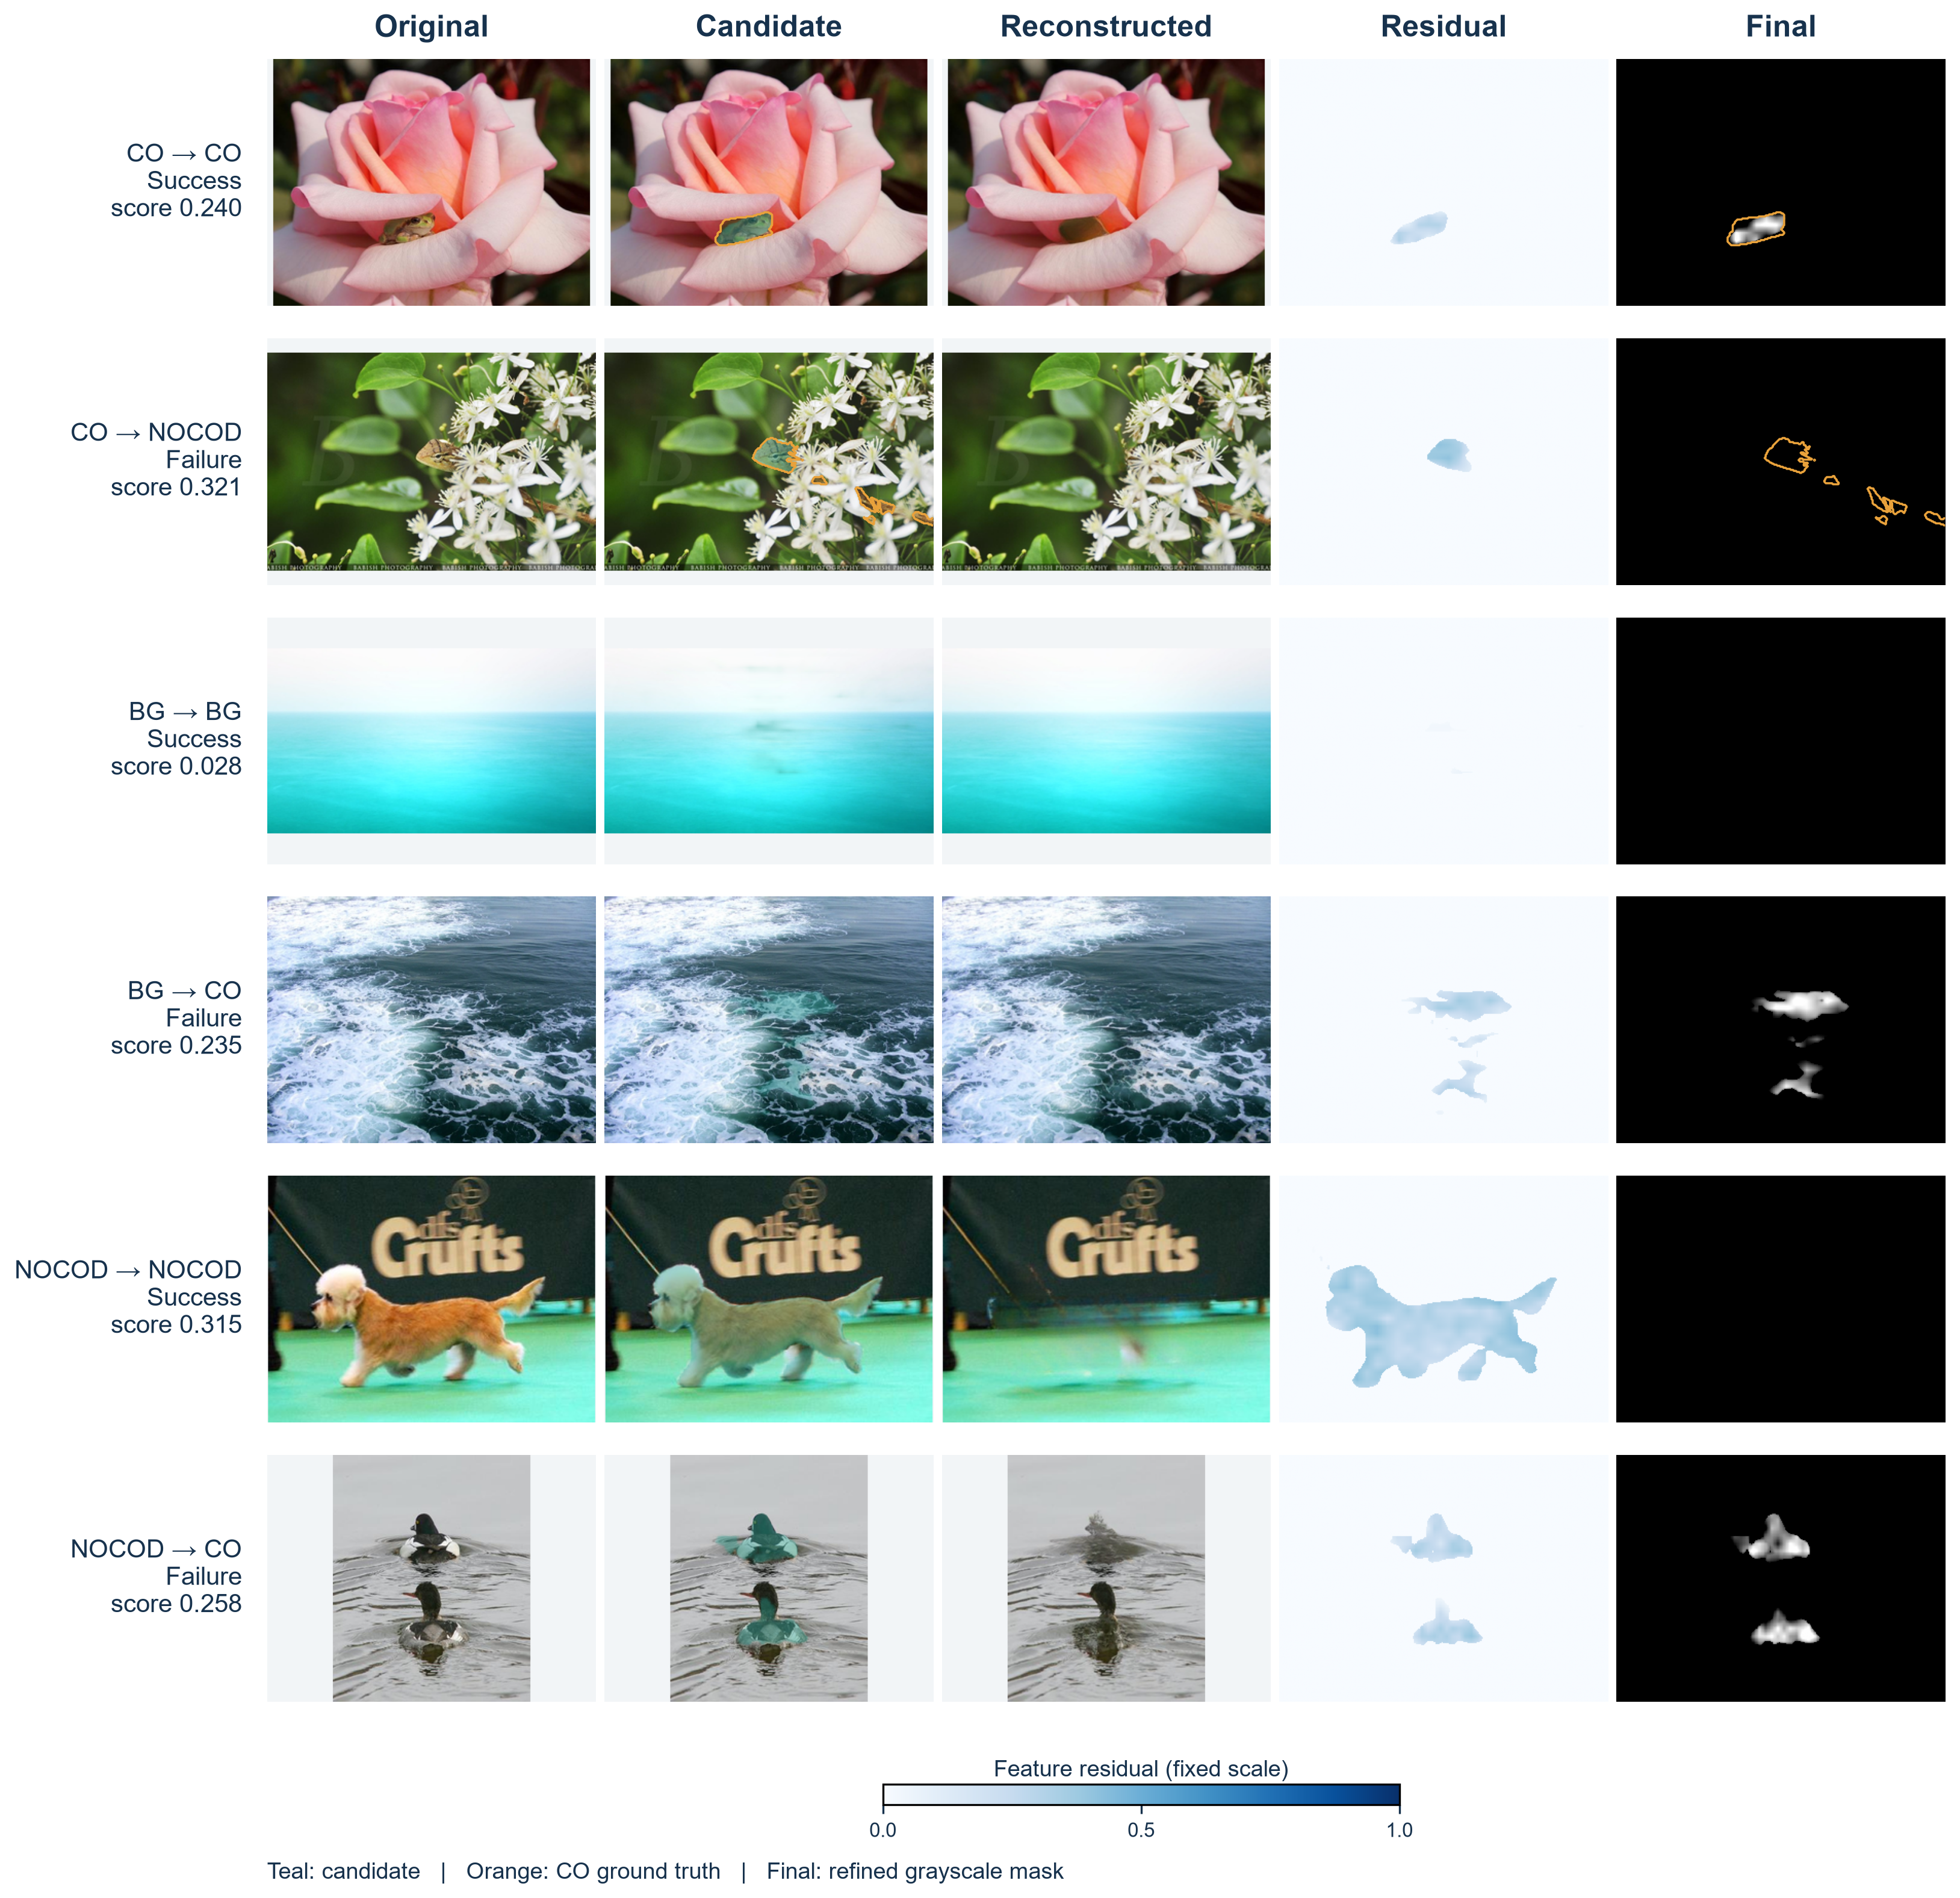
\includegraphics[width=0.94\textwidth]{figures/qualitative_cases.png}
\caption{Six real examples traced through the reconstruction and refinement pipeline.}
\label{fig:qualitative}

\end{figure}

\section{Comparison with recent literature}
\subsection{Realistic and open-world COD}
Table~\ref{tab:literature} compares OPC16K/OPCNet, USC12K/USCNet, and RCOD with our frozen, post-hoc verifier. Their tasks, outputs, training, and evaluation protocols differ, and no matched head-to-head experiment was conducted; the project therefore supports no superiority claim over these methods. RCOD's box annotations were downloaded but were not used as pixel-mask evaluation targets. \citep{opc16k,usc12k,rcod}

\subsection{Counterfactual and reconstruction-based methods}
CFCamo's paired detect-or-abstain training, Visual Jenga's object-dependency counterfactuals, and RUN's learned background extraction share aspects of reconstruction reasoning while answering distinct questions, as detailed in Table~\ref{tab:literature}. Their reported metrics cannot be ranked against this project's three-way USC12K accuracy without a harmonized protocol. The surveys reinforce why target-present segmentation alone cannot establish open-world presence decisions or source-independent transfer. \citep{cfcamo,visualjenga,run,xiaoSurvey,zhaoSurvey}

\begin{table}[htbp]
\centering
\small\caption{Research scope and comparability of recent related work.}
\label{tab:literature}
\begin{tabularx}{\textwidth}{L{2.5cm} L{4.1cm} Y}
\toprule
\textbf{Work} & \textbf{Method/question} & \textbf{Relation to this project} \\
\midrule
OPC16K / OPCNet & CO/BG/NOCOD benchmark and learned presence-aware segmentation & Hierarchical existence reasoning; our accuracy 0.7122 is on USC12K, not OPC16K; its release was unavailable at acquisition. \\
USC12K / USCNet & Joint salient/camouflaged scene reasoning and segmentation & End-to-end inter/intra-sample prompt queries; our feature-only band does not implement its aspect-relation module. \\
RCOD & Realistic camouflaged-object detection with box outputs and CAFR & Related realism objective, but box detection differs from our pixel-mask and three-class outputs. \\
CFCamo & Paired counterfactual detect-or-abstain policy & CF-COD Pair Accuracy 80.0--90.8\%; a different paired benchmark/metric, with explicit counterfactual supervision and policy training. \\
Visual Jenga & Counterfactual inpainting for object dependencies & Progressive object removal probes dependency and scene coherence, rather than camouflage presence. \\
RUN & Learned reversible RGB/mask unfolding with background extraction & Reversible RGB/mask unfolding integrates reconstruction-oriented background extraction into a trained segmenter. \\
\bottomrule
\end{tabularx}
\end{table}

\section{Revisiting the proposal's questions and assumptions}
The proposal's central ideas receive mixed support. The strongest positive result is not segmentation improvement; it is that a simple feature-only post-hoc layer can suppress many nonempty raw candidates on the negative classes. The most important negative result is that the class/source association and the CO-versus-NOCOD confusion prevent an interpretation as reliable, source-independent camouflage understanding. Table~\ref{tab:rqs} makes each judgment explicit.
\begin{table}[htbp]
\centering
\caption{Evidence-based answers to the original proposal.}
\label{tab:rqs}
\small
\begin{tabularx}{\textwidth}{L{3.6cm}L{2.2cm}Y}
\toprule
\textbf{Proposal question} & \textbf{Assessment} & \textbf{Evidence-based answer} \\
\midrule
Can reconstruction discrepancy distinguish CO, BG, and NOCOD? & Partially supported & A frozen two-cut feature band reached 0.7122 three-way accuracy on the saved evaluation split; class/source confounding and CO--NOCOD errors prevent a semantic or source-independent interpretation. \\
Which residual is most informative? & Partially supported & The ResNet feature residual was useful enough to calibrate a three-way rule, while the original composite direction failed a same-source check and had overfit weights. No controlled source-independent comparison establishes a generally best signal. \\
Can verification reduce false positives without harming CO segmentation? & Partially supported & Negative false acceptance dropped from 1.0000 for nonempty raw candidates to 0.2883 after verification, but raw masks score higher on three of four PySODMetrics measures and the verifier does not preserve CO mask quality. \\
Can residual-guided mask refinement improve boundaries? & Not supported & Refine improves neither the full set of reported segmentation measures nor the best raw baseline: S-alpha, weighted F-beta, and MAE are worse than raw. \\
Can the project compare against existence-aware/detect-or-abstain baselines? & Not answered & USCNet, OPCNet, and CFCamo were reviewed but not run under a matched protocol. No direct superiority claim is supported. \\
Does the pipeline provide a practical lightweight add-on? & Partially supported & The decision layer is frozen and simple, but the saved CPU run required $2.216\times10^4$ seconds total, including LaMa; cold-run wall time is material. \\
\bottomrule
\end{tabularx}

\par\smallskip{\footnotesize Assessment refers to this evaluated split and does not establish source-independent transfer.}
\end{table}


\section{Limitations and risks to the thesis claim}
\begin{enumerate}[leftmargin=2em]
\item \textbf{Source/class confounding.} In the USC12K training-derived pools used for development, eligible CO, BG, and NOCOD source families did not overlap. Thus training/holdout performance can reflect source style. The full split also preserves the benchmark's source-to-label construction. The same-source and transfer diagnostics exposed this risk, but do not remove it.
\item \textbf{Small calibration and holdout samples.} The three-way cuts were selected on 40 images per class and checked on 15 per class. The calibration and holdout accuracies were 0.708 and 0.667, respectively; uncertainty is considerable, and the samples do not support broad claims.
\item \textbf{Already-inspected evaluation split.} The 3,600-row official evaluation list has already been used for full-run reporting and post-hoc comparisons. Its bootstrap confidence intervals measure class-conditional sampling variation only, not a clean independent confirmation or robustness to a new source family.
\item \textbf{Segmentation tradeoff and metric correction.} On consistent PySODMetrics values, the raw masks outperform verify/refine on most CO metrics. The internal metric implementation was not suitable for final comparative claims, so this report uses the independent library output.
\item \textbf{Refinement is not established.} The refined outputs reduce negative mask area further, but CO segmentation quality declines on S-alpha, weighted F-beta, and MAE relative to raw masks. The higher adaptive E than verify does not offset the decline across the other measures.
\item \textbf{Runtime.} Fresh LaMa inpainting averaged 5.597485009890128 seconds per image on CPU in the saved run. The extra feature/reconstruction pass is therefore a substantial wall-clock cost for a post-hoc layer; a cached refinement timing is not representative of a cold run.
\item \textbf{No direct prior-work baseline.} No matched inference of USCNet, OPCNet, or an explicit existence-aware baseline was run. Comparison to their published results would be misleading because this project uses another model/checkpoint, class mapping, and evaluation setup.
\item \textbf{Band simplicity and label mapping.} The rule is a pair of scalar cuts on one pooled residual, ignores spatial residual structure for classification, and collapses USC12K's richer scene semantics into CO/BG/NOCOD. The band can label Scene-C images as CO even when salient content is also present.
\end{enumerate}

\section{Conclusion and honest assessment}
The work is substantive enough to support a master's thesis if the thesis is framed as an empirical study of counterfactual post-hoc verification, source confounds, negative rejection, and the detection/segmentation tradeoff. It is not sufficient evidence for a claim of a new state-of-the-art COD method, source-independent camouflage recognition, or segmentation enhancement. The strongest evidence-backed contribution is an audited experimental pipeline and a negative-rejection improvement over an operational raw-mask baseline on the saved USC12K evaluation split: mask-nonempty false acceptance falls from 1.0000 to 0.2883. Fair credit is due for implementing a genuine pretrained embedding residual, identifying a direction inversion rather than silently correcting it, preserving an independent development/holdout procedure before the full run, and validating the segmentation metric table with PySODMetrics.

The central conclusion should remain balanced: the verifier succeeds as a candidate rejection mechanism on this evaluated split, while the evidence does not show that it improves CO segmentation or generalizes independently of dataset source. That tension is a credible thesis result when reported transparently. For a stronger final thesis, the next research work should prioritize source-balanced or source-held-out data, compare against USCNet/OPCNet under their intended metrics once accessible, and pre-register an untouched evaluation design. These would be new experiments; none was run for this report.

\section*{Verification note}
The full run did not save previews. The authorized six-image supplement now exports original, candidate, reconstructed-background, residual, final-mask, and CO ground-truth stages using the original full-precision cache; no full-split evaluation was repeated. The report does not claim a fresh official test set: the saved manifest identifies the 3,600-image split as \texttt{usc12k\_official\_val}. OPC16K release status is stated only as documented by the project's acquisition-time \texttt{DATASETS.md}. The bibliography contains papers verified through author, conference, or arXiv records; no unverified citations or invented project results are used. The full split and post-hoc result have already been inspected, so all reported intervals are descriptive rather than confirmation on an untouched test set.

\FloatBarrier\begingroup\footnotesize\setlength{\bibsep}{2pt}\bibliographystyle{plainnat}
\bibliography{references}\endgroup
\appendix
\section{Data Provenance}\label{app:provenance}
\begingroup\smallAll source paths below are relative to the project root:\par
\path{C:/Users/a8aye/Documents/Codex/2026-09-23/there-is-a-proposal-file-in/outputs/counterfactual-cod}.
Displayed table values are rounded to four significant digits; unchanged integer counts are exact. Full precision is retained in \path{tables/full_precision_results.json} and \path{tables/pysodmetrics_full_precision.csv} within this report folder, as well as the original artifacts below.

\smallskip
\begin{tabularx}{\textwidth}{L{6.3cm}Y}
\toprule
\textbf{Report item} & \textbf{Source identifiers below} \\
\midrule
Table~\ref{tab:calibration}; Section 2.3 & D1, D3--D8 \\
Table~\ref{tab:classification}; headline metrics and intervals & D9--D10 \\
Table~\ref{tab:negativearea}; raw nonempty-mask baseline & D9--D11 \\
Table~\ref{tab:pysod}; Figure~\ref{fig:pysod}; segmentation comparison & D12 \\
Table~\ref{tab:literature}; Section 4 & Verified citations in \path{references.bib}; D1 for acquisition status \\
Table~\ref{tab:rqs}; proposal assessment & D0, D3--D12 \\
Table~\ref{tab:confusion}; Figure~\ref{fig:confusion} & D10 \\
Figure~\ref{fig:pipeline}; method and cuts & D1, D7, D9 \\
Figure~\ref{fig:qualitative}; six-image supplement & D2, D11, D13 \\
Dataset counts / mapping; timing / bootstrap procedure & D2; D9--D10 (2,000 replicates, seed 20261001) \\
\bottomrule
\end{tabularx}

\smallskip
{\footnotesize
\textbf{D0. Original proposal (absolute path).}\par
\path{C:/Users/a8aye/OneDrive/Desktop/Master/Term 4/Research_Project/project_proposal_draft_4.pdf}\par
\textbf{D1. Implementation and acquisition record.}\quad\path{README.md}; \path{DATASETS.md}\par
\textbf{D2. Official evaluation manifest.}\par
\path{data/experiments/usc12k/full/val_manifest.csv}\par
\textbf{D3. Initial class/source diagnosis.}\par
\path{data/experiments/usc12k/validation/calibration/class_structure/CLASS_DIAGNOSTICS.md}\par
\textbf{D4. COD10K matched diagnostic.}\par
\path{data/experiments/cod10k_matched/analysis/MATCHED_DIAGNOSTICS.md}\par
\textbf{D5. Fresh feature rule.}\par
\path{data/experiments/cod10k_feature_only/calibration/FEATURE_RULE.md}\par
\textbf{D6. USC-source feature sanity check.}\par
\path{data/experiments/cod10k_feature_only/usc_sanity/FEATURE_SANITY.md}\par
\textbf{D7. USC band calibration.}\par
\path{data/experiments/usc12k_feature_band/calibration/BAND_CALIBRATION.md}\par
\textbf{D8. Frozen band holdout.}\par
\path{data/experiments/usc12k_feature_band/heldout/USC_BAND_HOLDOUT.md}\par
\textbf{D9. Official run summaries (decision, counts, areas, timing).}\par
\path{data/experiments/usc12k/full/feature_band_lama_full/feature_band_verify/summary.json}\par
\path{data/experiments/usc12k/full/feature_band_lama_full/feature_band_refine/summary.json}\par
\textbf{D10. Classification and stratified-bootstrap estimates.}\par
\path{data/experiments/usc12k/full/feature_band_lama_full/posthoc_analysis/posthoc_summary.json}\par
\textbf{D11. Per-image mask areas and class decisions.}\par
\path{data/experiments/usc12k/full/feature_band_lama_full/posthoc_analysis/posthoc_per_image.csv}\par
\textbf{D12. Canonical segmentation table and validation protocol.}\par
\path{data/experiments/usc12k/full/feature_band_lama_full/posthoc_analysis/pysodmetrics_three_condition_table.csv}\par
\path{data/experiments/usc12k/full/feature_band_lama_full/posthoc_analysis/pysodmetrics_validation.json}\par
\path{data/experiments/usc12k/full/feature_band_lama_full/posthoc_analysis/PYSODMETRICS_VALIDATION.md}\par
\textbf{D13. Exact illustrative cases, supplementary outputs, and consistency audit.}\par
\path{reports/final_project_report/tables/qualitative_cases.csv}\par
\path{reports/final_project_report/supplementary/manifest.csv}\par
\path{reports/final_project_report/supplementary/refine/per_image.csv}\par
\path{reports/final_project_report/supplementary/refine/summary.json}\par
\path{reports/final_project_report/supplementary/consistency_check.json}\par
Stage images: \path{reports/final_project_report/supplementary/refine/previews/}\par
Each filename is the exact image ID from the case CSV plus \path{_original.png}, \path{_candidate.png}, \path{_background.png}, \path{_residual.png}, \path{_final.png}, or (CO only) \path{_ground_truth.png}. The original full-run cache is \path{data/experiments/usc12k/full/feature_band_lama_full/_residual_cache/}. The saved supplementary timer was 2.5894793999905232 seconds; all six cache entries were hits. Cached historical inpainting timings are not new inference timings.
}

\endgroup
\section{Exact confusion counts}\label{app:counts}
\begin{table}[H]
\centering
\caption{Exact full-split confusion counts.}
\label{tab:confusion}
\begin{tabular}{lrrr}
\toprule
\textbf{True / predicted} & \textbf{BG} & \textbf{CO} & \textbf{NOCOD} \\
\midrule
BG & 615 & 270 & 15 \\
CO & 141 & 1367 & 292 \\
NOCOD & 69 & 249 & 582 \\
\bottomrule
\end{tabular}

\par\smallskip{\footnotesize True rows; predicted columns. Source mapping: Appendix~\ref{app:provenance}.}
\end{table}

\end{document}
